\documentclass[10pt,twocolumn,letterpaper]{article}

\usepackage{cvpr}
\usepackage{times}
\usepackage{epsfig}
\usepackage{graphicx}
\usepackage{amsmath}
\usepackage{amssymb}
\usepackage{caption}
\usepackage{subcaption}
\usepackage[ruled,noline]{algorithm2e}

% Include other packages here, before hyperref.

% If you comment hyperref and then uncomment it, you should delete
% egpaper.aux before re-running latex.  (Or just hit 'q' on the first latex
% run, let it finish, and you should be clear).
%\usepackage[breaklinks=true,bookmarks=false]{hyperref}
\usepackage[pagebackref=true,breaklinks=true,letterpaper=true,colorlinks,bookmarks=false]{hyperref}

\SetKwInput{KwInput}{Input}
\SetKwInput{KwOutput}{Output}

\cvprfinalcopy % *** Uncomment this line for the final submission

\def\cvprPaperID{****} % *** Enter the CVPR Paper ID here
\def\httilde{\mbox{\tt\raisebox{-.5ex}{\symbol{126}}}}

% Pages are numbered in submission mode, and unnumbered in camera-ready
%\ifcvprfinal\pagestyle{empty}\fi
\setcounter{page}{1}
\begin{document}

%%%%%%%%% TITLE
%\title{\LaTeX\ Author Guidelines for CVPR Proceedings}
\title{{\vspace{-30mm}\small EECS 592 Advanced AI, Winter 2014, Project Progress Report} \\
~\\
~\\
~\\
~\\
Replication Studies on a State-of-the-art Part-based Human Detector}

%\author{First Author\\
%Institution1\\
%Institution1 address\\
%{\tt\small firstauthor@i1.org}
\author{Yu-Wei Chao\\
Department of Electrical Engineering and Computer Science \\
University of Michigan, Ann Arbor, MI 48109, USA\\
{\tt\small ywchao@umich}
% For a paper whose authors are all at the same institution,
% omit the following lines up until the closing ``}''.
% Additional authors and addresses can be added with ``\and'',
% just like the second author.
% To save space, use either the email address or home page, not both
%\and
%Second Author\\
%Institution2\\
%First line of institution2 address\\
%{\tt\small secondauthor@i2.org}
}

\maketitle
%\thispagestyle{empty}

%\begin{abstract}
%\end{abstract}

%\section{Introduction}
% Scene understanding/layout Estimation
Enabling machines to understand the visual scenes has been a major problem of computer vision research. Recently there has been a significant amount of works focusing on solving the spatial layouts of indoor scenes \cite{Hedau_ICCV2009,Lee_NIPS2010,Lee_CVPR2009,Schwing_CVPR2012,Wang_ECCV2010}. Estimating indoor spatial layouts leads to numerous applications, including robot navigation and scene recognition. Given an image of a room, as shown in Fig. \ref{fig:f1}, we want the computer to automatically identify the extent the floor, walls, and the ceiling (labeled by blue lines). \cite{Lee_CVPR2009} relies on the robust detection of straight lines to recover the boundaries between these planar surfaces. However, these boundaries are no longer observable if the scene is cluttered, as shown in Fig \ref{fig:f1}. To recover the spatial layout of cluttered rooms, \cite{Hedau_ICCV2009} jointly models the cluttered regions and the box model.

%Consider the image shown in Fig. \ref{fig:f1}, recent works on indoor scene understanding have focused on the following two tasks: 1) detecting semantic objects in the scene, such as furniture and human (red and green boxes), and 2) estimating the spatial layout (blue lines) \cite{Hedau_ICCV2009,Lee_NIPS2010,Lee_CVPR2009}.

% Object detection
Object detection is widely used for boosting the performance of scene understanding \cite{Bao_CVPR2010,Lee_NIPS2010}. \cite{Bao_CVPR2010} attempts to use the 3D locations of detected objects to help estimating the geometric properties of the scene. \cite{Lee_NIPS2010} explicitly models the relationship between the objects presented in the scene and the scene layout. However, in highly cluttered indoor scenes, object detections are often suffered by truncations and occlusions. As shown in Fig \ref{fig:f1} (red boxes), the dining table in the middle is partially occluded by the people in the front, while the chairs behind the dining table is almost non-visible due to the occlusion of the dining table and the people sitting on it. Furthermore, the chairs in the front are truncated by the image boundary. Objects cannot be robustly detected in these cases.

Thanks for the recent advances in human pose estimation and detection, human, as shown in Fig \ref{fig:f1} (green boxes) can be detected more robustly than objects in these circumstances. In this paper, we exploit human detection and 3D geometric information to solve the 3D layout of indoor scenes that is highly cluttered by objects and human.

% Contribution
\textbf{Contributions:} 1) we propose an unified framework for estimating three principle vanishing points of an indoor scene using human detection and 3D geometric information, 2) we propose a indoor scene dataset composed of images which are highly cluttered by objects and human, along with the annotations of layouts, objects, and human, and 3) we evaluate our method on the proposed dataset, and show state-of-the-art performance in vanishing point estimation and scene layout estimation.

The remaining of the proposal is organized as follows: Sec. \ref{sec:2} reviews the overall framework of our layout estimation method. We detail our proposed vanishing point estimation approach in Sec. \ref{sec:3}. Once we get three orthogonal vanishing points, we generate the candidate layouts and solve for the best, as described in Sec. \ref{sec:4} Sec. \ref{sec:5} presents the experimental design that we plan to perform. The milestones are listed in Sec. \ref{sec:6}.

\begin{figure}[t]
  \centering
  \begin{subfigure}[b]{0.23\textwidth}
    \centering
    \includegraphics[width=\textwidth]{figure/fig1-1.pdf}
    \label{fig:f1_1}
  \end{subfigure}
  ~
  \begin{subfigure}[b]{0.23\textwidth}
    \centering
    \includegraphics[width=1.05\textwidth]{figure/fig1-2.pdf}
    \label{fig:f1_2}
  \end{subfigure}
  \caption{In images of cluttered rooms, objects (red boxes) such as dining tables and chairs often suffer from occlusion and truncation, which are less robust to detect. We use the robustly detected human (green boxes) to jointly estimate the 3D box layout (blue lines) and human in their 3D locations.}
  \label{fig:f1}
\end{figure}

%\section{Estimating Room Layout}
\label{sec:2}

We follow \cite{Hedau_ICCV2009} to model the room by a 3D box. In each scene, we can observe at most five faces of the box model: floor, ceiling, and left, center, right walls. Following the Manhattan world assumption, each pair of the faces are either parallel or perpendicular to each other in 3D. The projection of each of these faces on the image are polygons, as shown in Fig. \ref{fig:f2}. The goal of layout estimation is to identify the boundaries between two faces, i.e. edges of polygons, within the image, and the recover the 3D box structure of the room.

Our approach follow the procedure of \cite{Hedau_ICCV2009,Lee_CVPR2009} to generate the layout of the room. First, we estimate the three orthogonal vanishing points of the box to get the box orientation (Sec. \ref{sec:3}). Different from \cite{Hedau_ICCV2009}, which estimate the vanishing points completely from 2D image features, i.e. line segments, our method exploits the 3D geometric relationship between human and the box, which jointly infers the vanishing points, camera pose and height, and human 3D locations. Next, we generate layout hypotheses by translating and scaling the faces of the box, and solve the best candidate layout based on \cite{Hedau_ICCV2009} (Sec. \ref{sec:4}).

\begin{figure}[t]
  \centering
  \hspace{-7mm}
  \begin{subfigure}[b]{0.21\textwidth}
    \centering
    \includegraphics[width=\textwidth]{figure/fig2-1.jpg}
    \label{fig:f2_1}
  \end{subfigure}
  ~
  \begin{subfigure}[b]{0.21\textwidth}
    \centering
    \includegraphics[width=1.13\textwidth]{figure/fig2-2.jpg}
    \label{fig:f2_2}
  \end{subfigure}
  \caption{Estimation room layouts.}
  \label{fig:f2}
\end{figure}
%\section{Vanishing Point Estimation from Human Detection and 3D Geometric Information}
\label{sec:3}

We propose a unified framework estimating three orthogonal vanishing points using candidate human bounding boxes and 3D geometric relationships. We first introduce our energy maximization framework in Sec. \ref{sec:3-1}. Then we detail each component of our model in Sec. \ref{sec:3-2}. We will describe how we solve the optimization in Sec. \ref{sec:3-3}.

\subsection{The Model}
\label{sec:3-1}
% Energy minimization\\
Given an observed image $I$, our goal is to jointly estimate human location $H$ and scene information $S$. Denote scene information $S = \{f,\phi,\psi,\omega,h\}$, where $f$ is the camera focal length, $\phi$, $\psi$, $\omega$ is the pitch, yaw, roll angle of the camera, and $h$ is the camera height. Note that the coordinates of three orthogonal vanishing points can be uniquely determined by $S = \{f,\phi,\psi,\omega\}$, and vice versa \cite{Hartley2004}. Suppose we obtain $N$ candidate human detections from the detector, we can denote  $H = \{H_i | i = 1,\dots,N\} = \{b_i, t_i | i = 1,\dots,N\}$, where $b_i$ is the detection bounding box and $t_i$ is the true positive flag of the $i$th candidate detection. We formulate the estimation of $H$ and $S$ as an energy maximization framework:
\begin{equation}
\begin{split}
  E(S,H,I) & = \alpha\Psi(S,H) + \beta\Psi(I,H) +\gamma\Psi(I,S) \\
           % & = \alpha\frac{1}{N}\sum_{i=1}^N\Psi(S,H_i) + \beta\frac{1}{N}\sum_{i=1}^N\Psi(I,H_i) + \gamma\Psi(I,S),
\end{split}
\end{equation}
where $\Psi(S,H)$ accounts for the compatibility between the scene hypothesis and human locations, $\Psi(I,H)$ measures the compatibility between the observed image and human locations, and $\Psi(I,S)$ measures the compatibility between the observed image and the scene hypothesis. $\alpha$, $\beta$, and $\gamma$ are the model parameters that weight each component.

\subsection{Model Characteristics}
\label{sec:3-2}
% Explain each term in detail\\
Now we explain each component of the model. Note that we assume the human positions are independent in the scene.

$\Psi(S,H) = \frac{1}{N}\sum_{i=1}^N\Psi(S,H_i)$ measure how likely the candidate detections to be a true positives with the scene information $S$. Given $S$, we first back-project the $i$th human detections onto the ground plane, assuming the human and the ground plane have the same normal. Denote the $g_i$ to be the 3D height of the $i$th candidate detection, we define $\Psi(S,H_i) = \ln\mathcal{N}(g_i-\mu_g,\sigma_g)$.

$\Psi(I,H) = \frac{1}{N}\sum_{i=1}^N\Psi(I,H_i)$ and we define $\Psi(I,H_i)$ to be the confidence of the $i$th candidate detection returned by the human detector.

$\Psi(I,S)$ measures the coherence between the observed line features and the vanishing points computed from scene hypothesis. As in \cite{Hedau_ICCV2009}, we first detect long straight lines in the image, then we compute the votes of each vanishing point from the lines using the exponential voting scheme. $\Psi(I,S)$ is set to be the sum of votes of three vanishing points.

\subsection{Solving Optimization}
\label{sec:3-3}
Since we explicitly model the camera and scene parameters, we can discretize the possible range of the parameter space, and enumerate through all the values for the optimum parameters. We will show that using a coarse discretization, our method is computational feasible, and outperforms the state-of-the-art approach in vanishing point estimation.

%\section{Generate and Evaluate Layout Hypotheses}
\label{sec:4}

Our initial plan for generating and evaluating candidate layouts is to follow the method described in \cite{Hedau_ICCV2009}. However, given the rich 3D scene information we obtain from vanishing point estimation, we can further refine the layout estimation which only relies on 2D features. We plan to combine the learned layout model in \cite{Hedau_ICCV2009} and our scene information $S$ to re-rank the candidate layouts, and obtain the final result.

%\section{Experimental Design}
\label{sec:5}

We aim to evaluate our algorithm on highly-cluttered indoor images with human presented. Since there is no available dataset satisfies our need, we will propose a new dataset that we call the \textit{indoor-human-activity} dataset for our evaluation. The \textit{indoor-human-activity} dataset will contains 911 images, and is composed of five human activity classes: dancing (187), having dinner (183), talking (193), washing dishes (183), and watching TV (165). Fig. \ref{fig:f5-1} shows sample images of the dataset. We will obtain a thorough annotation for objects, humans, and the layout for the dataset.

We plan to apply poselet detector \cite{Bourdev_ICCV2009,Bourdev_ECCV2010} to provide candidate human bounding boxes. To handle different human poses, we classify each candidate detection into two poses: standing and sitting, and assign different 3D CAD models for each pose. The classifier is trained by LIBSVM \cite{CC01a}. We adopt 50 images from each activity class for training the human pose classifier, and use the rest for evaluating the layout estimation. We consider the predicted human bounding boxes that have more than 50\% overlap with certain ground-truth bounding boxes to be our training data. We use the weighted poselet activation vector and the height ratio between full body and torso as the feature to train the SVM. We also plan to show some result of object detection on the dataset, and argue that objects can not be detected robustly.

We first evaluate the accuracy of vanishing point estimation (Sec \ref{sec:5-1}). In Sec \ref{sec:5-2}, we first show better estimated vanishing points can generate better candidate layout hypotheses, and then we analyze the contribution of layout estimation error by input vanishing points.


\subsection{Vanishing Point Estimation}
\label{sec:5-1}
Given three orthogonal vanishing points, we can calculate the pitch, yaw, roll angles, and the focal length of the camera. We adopt these values as the metrics of our evaluation. 

We compare the results of following methods.
\begin{itemize}
  \item Hedau's method \cite{Hedau_ICCV2009}
  \item Our partial method (w/o human): only $\Psi(I,S)$
  \item Our full method with GT human bounding boxes
  \item Our full method with poselet detections
  %\item Our full method (apply prior on scene parameters)
\end{itemize}

\subsection{Room Layout Estimation}
\label{sec:5-2}
First we analyze the candidate layouts generated by \cite{Hedau_ICCV2009} given three orthogonal vanishing points. We show that by improving vanishing point estimation, the best candidate layout can achieved lower pixel error.

Next, we compare the layout estimation results (in pixel error) of following methods.
\begin{itemize}
  \item Using VPs given by Hedau's method \cite{Hedau_ICCV2009}
  \item Using ground-truth VPs
  \item Using VPs given by our full method
\end{itemize}

\begin{figure*}[t]
  \centering
  \begin{subfigure}[b]{0.20\textwidth}
    \centering
    \begin{subfigure}[b]{0.23\textwidth}
      \centering
      \centerline{\includegraphics[height=2.5\textwidth]{figure/sample_img/dc1.jpg}}
    \end{subfigure} \\
    ~\vspace{-3.0mm}\\
    \begin{subfigure}[b]{0.23\textwidth}
      \centering
      \centerline{\includegraphics[height=2.5\textwidth]{figure/sample_img/dc2.jpg}}
    \end{subfigure} \\
    ~\vspace{-3.0mm}\\
    \begin{subfigure}[b]{0.23\textwidth}
      \centering
      \centerline{\includegraphics[height=2.5\textwidth]{figure/sample_img/dc3.jpg}}
    \end{subfigure} \\
    ~\vspace{-3.0mm}\\
    \begin{subfigure}[b]{0.23\textwidth}
      \centering
      \centerline{\includegraphics[height=2.5\textwidth]{figure/sample_img/dc4.jpg}}
    \end{subfigure} \\
    \caption{dancing}
  \end{subfigure}
  ~\hspace{-3mm}
  \begin{subfigure}[b]{0.20\textwidth}
    \centering
    \begin{subfigure}[b]{0.23\textwidth}
      \centering
      \centerline{\includegraphics[height=2.5\textwidth]{figure/sample_img/hd1.jpg}}
    \end{subfigure} \\
    ~\vspace{-3.0mm}\\
    \begin{subfigure}[b]{0.23\textwidth}
      \centering
      \centerline{\includegraphics[height=2.5\textwidth]{figure/sample_img/hd2.jpg}}
    \end{subfigure} \\
    ~\vspace{-3.0mm}\\
    \begin{subfigure}[b]{0.23\textwidth}
      \centering
      \centerline{\includegraphics[height=2.5\textwidth]{figure/sample_img/hd3.jpg}}
    \end{subfigure} \\
    ~\vspace{-3.0mm}\\
    \begin{subfigure}[b]{0.23\textwidth}
      \centering
      \centerline{\includegraphics[height=2.5\textwidth]{figure/sample_img/hd4.jpg}}
    \end{subfigure} \\
    \caption{having dinner}
  \end{subfigure}
  ~\hspace{-3mm}
  \begin{subfigure}[b]{0.20\textwidth}
    \centering
    \begin{subfigure}[b]{0.23\textwidth}
      \centering
      \centerline{\includegraphics[height=2.5\textwidth]{figure/sample_img/tk1.jpg}}
    \end{subfigure} \\
    ~\vspace{-3.0mm}\\
    \begin{subfigure}[b]{0.23\textwidth}
      \centering
      \centerline{\includegraphics[height=2.5\textwidth]{figure/sample_img/tk2.jpg}}
    \end{subfigure} \\
    ~\vspace{-3.0mm}\\
    \begin{subfigure}[b]{0.23\textwidth}
      \centering
      \centerline{\includegraphics[height=2.5\textwidth]{figure/sample_img/tk3.jpg}}
    \end{subfigure} \\
    ~\vspace{-3.0mm}\\
    \begin{subfigure}[b]{0.23\textwidth}
      \centering
      \centerline{\includegraphics[height=2.5\textwidth]{figure/sample_img/tk4.jpg}}
    \end{subfigure} \\
    \caption{talking}
  \end{subfigure}
  ~\hspace{-3mm}
  \begin{subfigure}[b]{0.20\textwidth}
    \centering
    \begin{subfigure}[b]{0.23\textwidth}
      \centering
      \centerline{\includegraphics[height=2.5\textwidth]{figure/sample_img/wd1.jpg}}
    \end{subfigure} \\
    ~\vspace{-3.0mm}\\
    \begin{subfigure}[b]{0.23\textwidth}
      \centering
      \centerline{\includegraphics[height=2.5\textwidth]{figure/sample_img/wd2.jpg}}
    \end{subfigure} \\
    ~\vspace{-3.0mm}\\
    \begin{subfigure}[b]{0.23\textwidth}
      \centering
      \centerline{\includegraphics[height=2.5\textwidth]{figure/sample_img/wd3.jpg}}
    \end{subfigure} \\
    ~\vspace{-3.0mm}\\
    \begin{subfigure}[b]{0.23\textwidth}
      \centering
      \centerline{\includegraphics[height=2.5\textwidth]{figure/sample_img/wd4.jpg}}
    \end{subfigure} \\
    \caption{washing dishes}
  \end{subfigure}
  ~\hspace{-3mm}
  \begin{subfigure}[b]{0.20\textwidth}
    \centering
    \begin{subfigure}[b]{0.23\textwidth}
      \centering
      \centerline{\includegraphics[height=2.5\textwidth]{figure/sample_img/wt1.jpg}}
    \end{subfigure} \\
    ~\vspace{-3.0mm}\\
    \begin{subfigure}[b]{0.23\textwidth}
      \centering
      \centerline{\includegraphics[height=2.5\textwidth]{figure/sample_img/wt2.jpg}}
    \end{subfigure} \\
    ~\vspace{-3.0mm}\\
    \begin{subfigure}[b]{0.23\textwidth}
      \centering
      \centerline{\includegraphics[height=2.5\textwidth]{figure/sample_img/wt3.jpg}}
    \end{subfigure} \\
    ~\vspace{-3.0mm}\\
    \begin{subfigure}[b]{0.23\textwidth}
      \centering
      \centerline{\includegraphics[height=2.5\textwidth]{figure/sample_img/wt4.jpg}}
    \end{subfigure} \\
    \caption{watching TV}
  \end{subfigure}
  \caption{Sample images from our collected \textit{indoor-human-activity} dataset.}
  \label{fig:f5-1}
\end{figure*}
%\section{Milestones}
\label{sec:6}

The milestones are shown in Table \ref{tab:6}
\begin{table}[t]
  \centering
  \begin{tabular}{|l|p{5.5 cm}|}
    \hline
    Date          & Plan \\
    \hline
    02.12 - 02.18 & Experiments on VP estimation \\
    02.19 - 02.25 & Experiments on VP estimation \\
    02.26 - 03.04 & Experiments on layout estimation \\
    03.05 - 03.11 & Experiments on layout estimation \\
    03.12 - 03.18 & Possible extension - apply all scene parameters for layout estimation \\
    03.19 - 03.25 & Possible extension - apply all scene parameters for layout estimation \\
    03.26 - 04.01 & Possible extension - inference \\
    04.02 - 04.08 & Possible extension - inference \\
    04.09 - 04.15 & Buffer time \\
    04.16 - 04.22 & Buffer time \\
    04.23 - 04.29 & Prepare for presentation \\
    \hline
  \end{tabular}
  \caption{Milestones of the project}
  \label{tab:6}
\end{table}


%\input{02_relate}
%\input{03_layout}
%\input{04_vpest}
%\section{Experimental Design}
\label{sec:5}

We aim to evaluate our algorithm on highly-cluttered indoor images with human presented. Since there is no available dataset satisfies our need, we will propose a new dataset that we call the \textit{indoor-human-activity} dataset for our evaluation. The \textit{indoor-human-activity} dataset will contains 911 images, and is composed of five human activity classes: dancing (187), having dinner (183), talking (193), washing dishes (183), and watching TV (165). Fig. \ref{fig:f5-1} shows sample images of the dataset. We will obtain a thorough annotation for objects, humans, and the layout for the dataset.

We plan to apply poselet detector \cite{Bourdev_ICCV2009,Bourdev_ECCV2010} to provide candidate human bounding boxes. To handle different human poses, we classify each candidate detection into two poses: standing and sitting, and assign different 3D CAD models for each pose. The classifier is trained by LIBSVM \cite{CC01a}. We adopt 50 images from each activity class for training the human pose classifier, and use the rest for evaluating the layout estimation. We consider the predicted human bounding boxes that have more than 50\% overlap with certain ground-truth bounding boxes to be our training data. We use the weighted poselet activation vector and the height ratio between full body and torso as the feature to train the SVM. We also plan to show some result of object detection on the dataset, and argue that objects can not be detected robustly.

We first evaluate the accuracy of vanishing point estimation (Sec \ref{sec:5-1}). In Sec \ref{sec:5-2}, we first show better estimated vanishing points can generate better candidate layout hypotheses, and then we analyze the contribution of layout estimation error by input vanishing points.


\subsection{Vanishing Point Estimation}
\label{sec:5-1}
Given three orthogonal vanishing points, we can calculate the pitch, yaw, roll angles, and the focal length of the camera. We adopt these values as the metrics of our evaluation. 

We compare the results of following methods.
\begin{itemize}
  \item Hedau's method \cite{Hedau_ICCV2009}
  \item Our partial method (w/o human): only $\Psi(I,S)$
  \item Our full method with GT human bounding boxes
  \item Our full method with poselet detections
  %\item Our full method (apply prior on scene parameters)
\end{itemize}

\subsection{Room Layout Estimation}
\label{sec:5-2}
First we analyze the candidate layouts generated by \cite{Hedau_ICCV2009} given three orthogonal vanishing points. We show that by improving vanishing point estimation, the best candidate layout can achieved lower pixel error.

Next, we compare the layout estimation results (in pixel error) of following methods.
\begin{itemize}
  \item Using VPs given by Hedau's method \cite{Hedau_ICCV2009}
  \item Using ground-truth VPs
  \item Using VPs given by our full method
\end{itemize}

\begin{figure*}[t]
  \centering
  \begin{subfigure}[b]{0.20\textwidth}
    \centering
    \begin{subfigure}[b]{0.23\textwidth}
      \centering
      \centerline{\includegraphics[height=2.5\textwidth]{figure/sample_img/dc1.jpg}}
    \end{subfigure} \\
    ~\vspace{-3.0mm}\\
    \begin{subfigure}[b]{0.23\textwidth}
      \centering
      \centerline{\includegraphics[height=2.5\textwidth]{figure/sample_img/dc2.jpg}}
    \end{subfigure} \\
    ~\vspace{-3.0mm}\\
    \begin{subfigure}[b]{0.23\textwidth}
      \centering
      \centerline{\includegraphics[height=2.5\textwidth]{figure/sample_img/dc3.jpg}}
    \end{subfigure} \\
    ~\vspace{-3.0mm}\\
    \begin{subfigure}[b]{0.23\textwidth}
      \centering
      \centerline{\includegraphics[height=2.5\textwidth]{figure/sample_img/dc4.jpg}}
    \end{subfigure} \\
    \caption{dancing}
  \end{subfigure}
  ~\hspace{-3mm}
  \begin{subfigure}[b]{0.20\textwidth}
    \centering
    \begin{subfigure}[b]{0.23\textwidth}
      \centering
      \centerline{\includegraphics[height=2.5\textwidth]{figure/sample_img/hd1.jpg}}
    \end{subfigure} \\
    ~\vspace{-3.0mm}\\
    \begin{subfigure}[b]{0.23\textwidth}
      \centering
      \centerline{\includegraphics[height=2.5\textwidth]{figure/sample_img/hd2.jpg}}
    \end{subfigure} \\
    ~\vspace{-3.0mm}\\
    \begin{subfigure}[b]{0.23\textwidth}
      \centering
      \centerline{\includegraphics[height=2.5\textwidth]{figure/sample_img/hd3.jpg}}
    \end{subfigure} \\
    ~\vspace{-3.0mm}\\
    \begin{subfigure}[b]{0.23\textwidth}
      \centering
      \centerline{\includegraphics[height=2.5\textwidth]{figure/sample_img/hd4.jpg}}
    \end{subfigure} \\
    \caption{having dinner}
  \end{subfigure}
  ~\hspace{-3mm}
  \begin{subfigure}[b]{0.20\textwidth}
    \centering
    \begin{subfigure}[b]{0.23\textwidth}
      \centering
      \centerline{\includegraphics[height=2.5\textwidth]{figure/sample_img/tk1.jpg}}
    \end{subfigure} \\
    ~\vspace{-3.0mm}\\
    \begin{subfigure}[b]{0.23\textwidth}
      \centering
      \centerline{\includegraphics[height=2.5\textwidth]{figure/sample_img/tk2.jpg}}
    \end{subfigure} \\
    ~\vspace{-3.0mm}\\
    \begin{subfigure}[b]{0.23\textwidth}
      \centering
      \centerline{\includegraphics[height=2.5\textwidth]{figure/sample_img/tk3.jpg}}
    \end{subfigure} \\
    ~\vspace{-3.0mm}\\
    \begin{subfigure}[b]{0.23\textwidth}
      \centering
      \centerline{\includegraphics[height=2.5\textwidth]{figure/sample_img/tk4.jpg}}
    \end{subfigure} \\
    \caption{talking}
  \end{subfigure}
  ~\hspace{-3mm}
  \begin{subfigure}[b]{0.20\textwidth}
    \centering
    \begin{subfigure}[b]{0.23\textwidth}
      \centering
      \centerline{\includegraphics[height=2.5\textwidth]{figure/sample_img/wd1.jpg}}
    \end{subfigure} \\
    ~\vspace{-3.0mm}\\
    \begin{subfigure}[b]{0.23\textwidth}
      \centering
      \centerline{\includegraphics[height=2.5\textwidth]{figure/sample_img/wd2.jpg}}
    \end{subfigure} \\
    ~\vspace{-3.0mm}\\
    \begin{subfigure}[b]{0.23\textwidth}
      \centering
      \centerline{\includegraphics[height=2.5\textwidth]{figure/sample_img/wd3.jpg}}
    \end{subfigure} \\
    ~\vspace{-3.0mm}\\
    \begin{subfigure}[b]{0.23\textwidth}
      \centering
      \centerline{\includegraphics[height=2.5\textwidth]{figure/sample_img/wd4.jpg}}
    \end{subfigure} \\
    \caption{washing dishes}
  \end{subfigure}
  ~\hspace{-3mm}
  \begin{subfigure}[b]{0.20\textwidth}
    \centering
    \begin{subfigure}[b]{0.23\textwidth}
      \centering
      \centerline{\includegraphics[height=2.5\textwidth]{figure/sample_img/wt1.jpg}}
    \end{subfigure} \\
    ~\vspace{-3.0mm}\\
    \begin{subfigure}[b]{0.23\textwidth}
      \centering
      \centerline{\includegraphics[height=2.5\textwidth]{figure/sample_img/wt2.jpg}}
    \end{subfigure} \\
    ~\vspace{-3.0mm}\\
    \begin{subfigure}[b]{0.23\textwidth}
      \centering
      \centerline{\includegraphics[height=2.5\textwidth]{figure/sample_img/wt3.jpg}}
    \end{subfigure} \\
    ~\vspace{-3.0mm}\\
    \begin{subfigure}[b]{0.23\textwidth}
      \centering
      \centerline{\includegraphics[height=2.5\textwidth]{figure/sample_img/wt4.jpg}}
    \end{subfigure} \\
    \caption{watching TV}
  \end{subfigure}
  \caption{Sample images from our collected \textit{indoor-human-activity} dataset.}
  \label{fig:f5-1}
\end{figure*}
%\input{06_conclude}

\section{Introduction}
\begin{figure}[t]
  \centering
  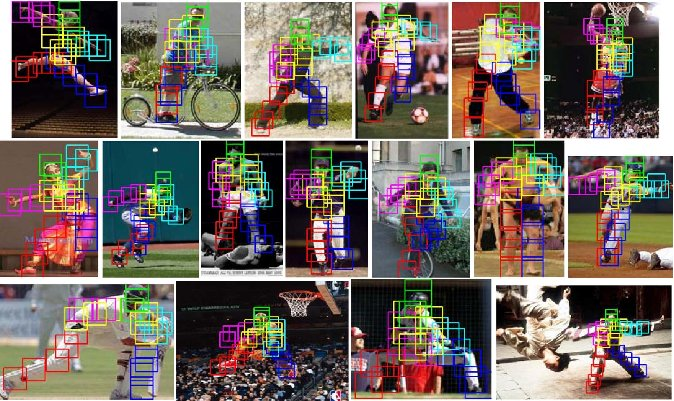
\includegraphics[width=8.3cm]{figure/parse_results.jpg}
  \caption{Illustration of Yang and Ramanan's work on human detection and pose estimation \cite{Yang_PAMI2011}. Different color of boxes identify different local parts of human body.}
\label{fig:intro}
\end{figure}
Human detection and pose estimation is a challenging problem in computer vision studies. Recently there has been many outstanding works published in addressing the these problems \cite{Bourdev_ICCV2009, Bourdev_ECCV2010, Felzenszwalb_PAMI2010, Yang_PAMI2011, Shotton_CVPR2011}. A very interesting line of work is the application of part-based models \cite{Felzenszwalb_PAMI2010, Yang_PAMI2011}. Part-based models can be viewed an extension of the rigid template models in the way that the target objects are represented by local parts, and the locations of these local parts have some amount of flexibility to capture the uncertainly in real-world data.

In this work, we proposed to replicate Yang and Ramanan's paper \cite{Yang_PAMI2011} on human detection and pose estimation. Unlike the famous deformable part-based model \cite{Felzenszwalb_PAMI2010}, which addressed generic object detection, Yang and Ramanan focus specifically on human detection in RGB images. They carefully designed a system that can locate the body parts of the human, as illustrated in Fig. \ref{fig:intro}. They used a mixtures of templates for each parts so they can effetively modeled human poses.

\section{Replication Plan}
\begin{figure}[t]
  \centering
  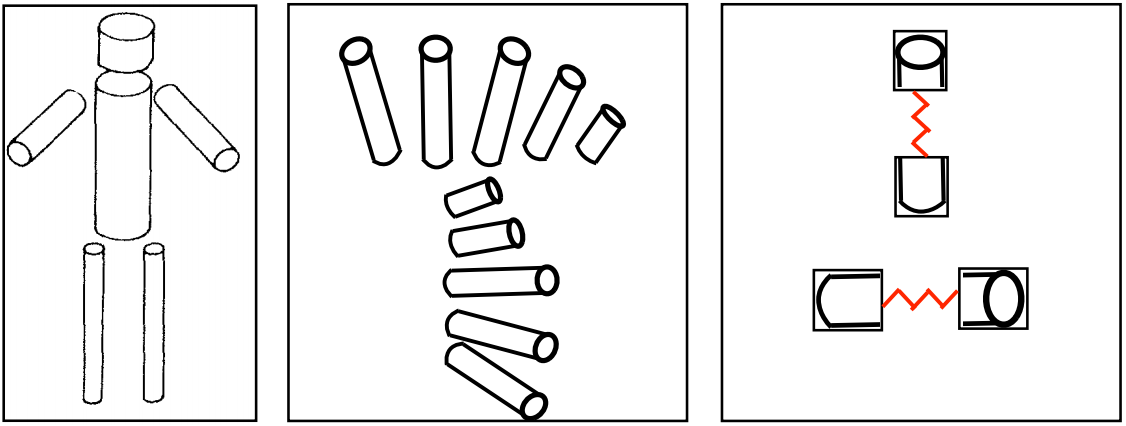
\includegraphics[width=8.3cm]{figure/pictorial.png}
  \caption{Illustration of the pictorial structure and mixture of local parts.}
\label{}
\end{figure}

We list our plans for this replication study as following:
\begin{itemize}
  \item Re-implement the inference algorithm. We plan to investigate the efficiency of the inference algorithm, which is not presented in the paper.
  \item Re-do the training process. The paper uses a fixed training set provided by the Image Parse dataset and the Buffy Stickman dataset. We plan to re-train the model with different settings, either using a subset or on a new dataset. The goal is to better understand how the trained model changes by different training settings. 
  \item Build on own human dataset. We can build a small but more challenging dataset, and see how far can the target method go.
  
\end{itemize}

\section{Inference}
We first briefly review the overall pictorial structure model for human detection proposed in \cite{Yang_PAMI2011} and the inference problem in Sec. \ref{sec:inference_ov}. Next we evaluate our implementation of the inference algorithm on the the Image Parse data \cite{Ramanan_NIPS2006} in Sec. \ref{sec:inference_eval}.

\subsection{Algorithm Overview}
\label{sec:inference_ov}
Yang \emph{et al.} proposed a pictorial structure representation to robustly model the human poses caused by articulated body configurations. They have a flexible design in the way that each local part is a mixture of different component (i.e. can be chosen from a template set). Let $I$ denote the image, $l_i = (x_i, y_i)$ be the location of part $i$, and $t_i$ be the mixture component of part $i$ (using the $t_i$th template for part $i$), where $i\in \{1,\dots,K\}$, $l_i\in\{1,\dots,L\}$, and $t_i\in\{1,\dots,T\}$. Assuming the human body is a tree structured graph $G=(V,E)$, the score function of a human is defined as following:
\begin{equation}
\label{eq:model}
  S(I,l,t) = \sum_{i\in V}\omega_i^{t_i}\cdot\phi(I,l_i) + \sum_{i,j\in E}\omega_{ij}^{t_i,t_j}\cdot\psi(l_i-l_j) + S(t).
\end{equation}
The three terms in eq. \ref{eq:model} correspond to the appearance model, deformation model, and the co-occurence model. Appreance model computes the local scores by placing a part template $w_i^{t_i}$ (of type $t_i$) at the location $i$. Deformation model controls the relative position of part $i$ and $j$. Note that $\psi(l_i-l_j)=[dx\text{~~}dx^{2}\text{~~}dy\text{~~}dy^{2}]^{\top}$. The co-occurrence model 
\begin{equation}
  S(t) = \sum_{i\in V}b_i^{t_i} + \sum_{i,j\in E}b_{ij}^{t_i,t_j}
\end{equation}
captures the occurrence likelihood of part $i$ with type $t_i$ and the co-occurrence likelihood of part $i$ with type $t_i$ and part $j$ with type $j$.

Given the model parameter, inference correspends to finding the maximum scoring locaions $(l,t)$ given the image $I$. Denote $z_i = (t_i,l_i)$, the eq \ref{eq:model} can be written as
\begin{equation}
  \begin{split}
    S(I,z) = & \sum_{i\in V}\phi_i(I,z_i) + \sum_{i,j\in E}\psi_{ij}(z_i,z_j), \\
    \text{where~~~~} & \phi_i(I,z_i) = \omega_i^{t_i}\cdot\phi(I,l_i)+b_i^{t_i} \\
                   & \psi_{ij}(z_i,z_j) = \omega_{ij}^{t_i,t_j}\cdot\psi(l_i-l_j)+b_{ij}^{t_i,t_j} \\
  \end{split}
\end{equation}
One nice consequence of the tree structure assumption on human body representation is enabling us to solve the optimization problem efficiently by dynamic programming.	Our first focus of this replication study is on re-implementing this inference algorithm.

\subsection{Evaluation}
\label{sec:inference_eval}
We verify our implementation by first comparing the result on the same benchmark dataset, Image Parse Dataset \cite{Ramanan_NIPS2006}. The dataset consists of 100 training images and 205 test images. Since we only want to verify our inference implementation, we use only the test images for experiment. As \cite{Ramanan_NIPS2006}, we evaluate the result using two different metrics: 1) probability of a correct keypoint (PCK), and 2) average precision of keypoints (APK). The comparison between our implementation and the original paper is reported in Table \ref{tab:pck_parse} and \ref{tab:apk_parse}. Note that the authors have made their code public online. Since we observe a difference in the result obtained by running their released code and the number they reported in \cite{Ramanan_NIPS2006}, we use the numbers obtained by their release code for comparison here.

For the quantitative evaluation, we observe a significant gap between our implementation and the author's implementation. This indicates that our implementation of inference clearly still contain mistakes. We also showed the qualitative examples for detected human in Fig. \ref{fig:inference_exp}. Looking through the example image, we see that the implementation actually works in a reasonbly good level. This suggests that the mistake might be minor. A good strategy for debugging the implementation will be comparing with the author's code by fixing the module of the algorithm one at a time. We plan to carry out that as our next step.

%\begin{algorithm}
%  \dontprintsemicolon
%  \KwInput{a}
%  \KwOutput{a}
%  \Begin{
%    $V \longleftarrow U$\;
%    $S \longleftarrow \emptyset$\;
%    \For{$x\in X$}{
%      $NbSuccInS(x) \longleftarrow 0$\;
%      $NbPredInMin(x) \longleftarrow 0$\;
%      $NbPredNotInMin(x) \longleftarrow |ImPred(x)|$\;
%    }
%    \For{$x \in X$}{
%      \If{$NbPredInMin(x) = 0$ {\bf and} $NbPredNotInMin(x) = 0$}{
%        $AppendToMin(x)$}
%    }
%    \While{$S \neq \emptyset$}{
%      \While{$|S \cap ImSucc(x)| \neq |S|$}{
%        \For{$ y \in S-ImSucc(x)$}{
%          \{ remove from $V$ all the arcs $zy$ : \}\;
%          \For{$z \in ImPred(y) \cap Min$}{
%            remove the arc $zy$ from $V$\;
%            $NbSuccInS(z) \longleftarrow NbSuccInS(z) - 1$\;
%            move $z$ in $T$ to the list preceding its present list\;
%            \{i.e. If $z \in T[k]$, move $z$ from $T[k]$ to
%            $T[k-1]$\}\;
%          }
%          $NbPredInMin(y) \longleftarrow 0$\;
%          $NbPredNotInMin(y) \longleftarrow 0$\;
%          $S \longleftarrow S - \{y\}$\;
%          $AppendToMin(y)$\;
%        }
%      }
%    $RemoveFromMin(x)$\;
%    }
%  }
%\caption{}
%\end{algorithm}

\begin{table}[t]
  \begin{center}
    \begin{tabular}{|p{0.8cm}|p{0.5cm}|p{0.5cm}|p{0.5cm}|p{0.5cm}|p{0.5cm}|p{0.5cm}|p{0.5cm}||p{0.5cm}|}
      \hline
      Parse                & Hea  & Sho  & Elb  & Wri  & Hip  & Kne  & Ank  & Avg  \\ \hline
      \hline
      \cite{Yang_PAMI2011} & 88.3 & 82.7 & 61.2 & 44.1 & 68.8 & 66.8 & 61.0 & 67.6 \\ \hline
      Mine                 & 77.3 & 71.2 & 47.3 & 31.7 & 58.8 & 56.8 & 49.3 & 56.1 \\ \hline
    \end{tabular}
  \end{center}
  \caption{Probability of correct keypoints (PCK) on the Image Parse Dataset.}
  \label{tab:pck_parse}
\end{table}

\begin{table}
  \begin{center}
    \begin{tabular}{|p{0.8cm}|p{0.5cm}|p{0.5cm}|p{0.5cm}|p{0.5cm}|p{0.5cm}|p{0.5cm}|p{0.5cm}||p{0.5cm}|}
      \hline
      Parse                & Hea  & Sho  & Elb  & Wri  & Hip  & Kne  & Ank  & Avg \\ \hline
      \hline
      \cite{Yang_PAMI2011} & 83.9 & 77.0 & 49.6 & 26.8 & 56.1 & 52.3 & 43.7 & 55.6 \\ \hline
      Mine                 & 71.2 & 62.8 & 32.4 & 15.8 & 42.9 & 38.8 & 33.1 & 42.4 \\ \hline
    \end{tabular}
  \end{center}
  \caption{Average precision of keypoints (APK) on the Image Parse Dataset.}
  \label{tab:apk_parse}
\end{table}

\begin{figure*}[b!]
  \begin{center}
    %\begin{tabular}{cccccc}
      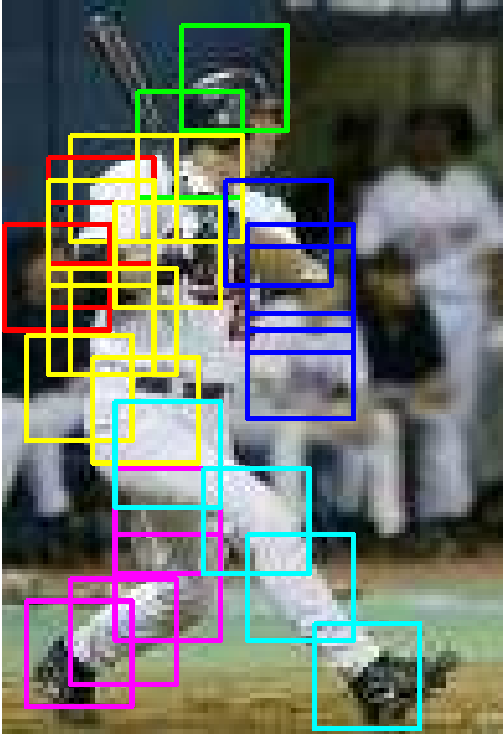
\includegraphics[height=0.164\linewidth]{figure/inference_example/img0003_1.pdf}~~%&
      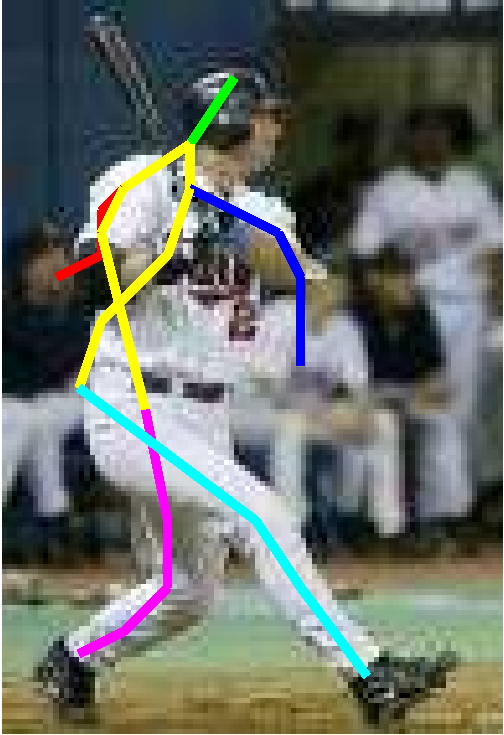
\includegraphics[height=0.164\linewidth]{figure/inference_example/img0003_2.pdf}~~%&
      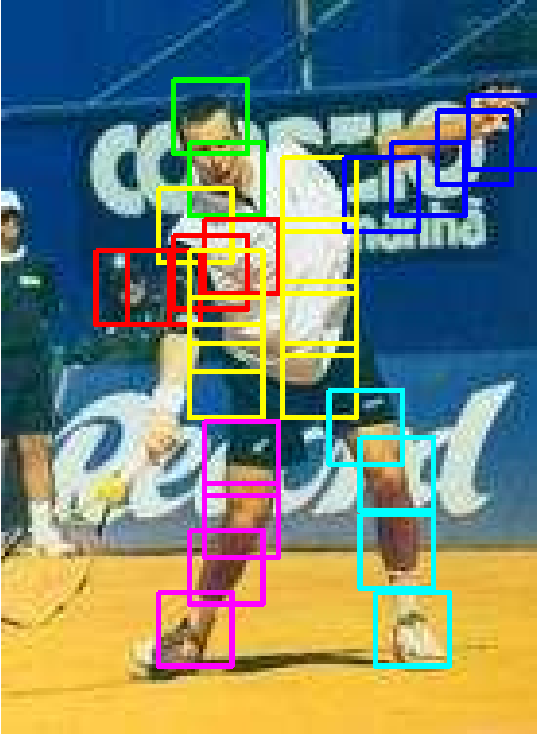
\includegraphics[height=0.164\linewidth]{figure/inference_example/img0005_1.pdf}~~%&
      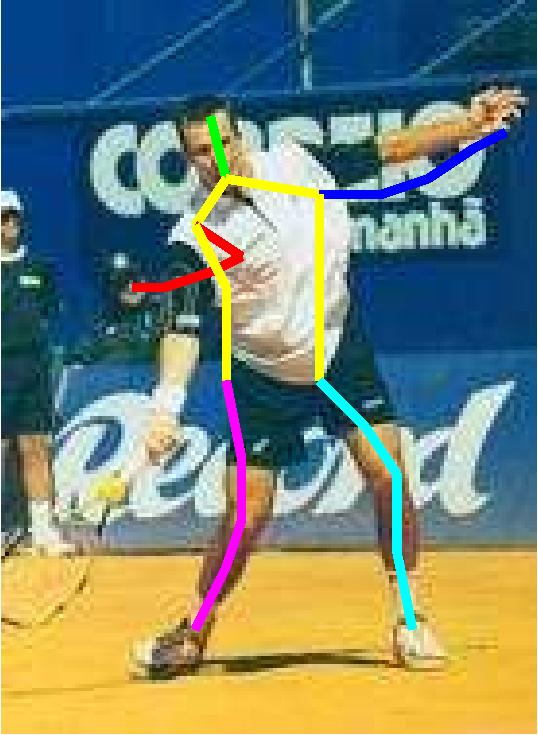
\includegraphics[height=0.164\linewidth]{figure/inference_example/img0005_2.pdf}~~%&
      \includegraphics[height=0.164\linewidth]{figure/inference_example/img0037_1.pdf}~~%&
      \includegraphics[height=0.164\linewidth]{figure/inference_example/img0037_2.pdf}~~\\
      \vspace{0.2cm}
      \includegraphics[height=0.144\linewidth]{figure/inference_example/img0016_1.pdf}~~%&
      \includegraphics[height=0.144\linewidth]{figure/inference_example/img0016_2.pdf}~~%&
      \includegraphics[height=0.144\linewidth]{figure/inference_example/img0149_1.pdf}~~%&
      \includegraphics[height=0.144\linewidth]{figure/inference_example/img0149_2.pdf}~~%&
      \includegraphics[height=0.144\linewidth]{figure/inference_example/img0175_1.pdf}~~%&
      \includegraphics[height=0.144\linewidth]{figure/inference_example/img0175_2.pdf}\\
      \vspace{0.2cm}
      \includegraphics[height=0.147\linewidth]{figure/inference_example/img0002_1.pdf}~~%&
      \includegraphics[height=0.147\linewidth]{figure/inference_example/img0002_2.pdf}~~~%&
      \includegraphics[height=0.147\linewidth]{figure/inference_example/img0010_1.pdf}~~%&
      \includegraphics[height=0.147\linewidth]{figure/inference_example/img0010_2.pdf}~~~%&
      \includegraphics[height=0.147\linewidth]{figure/inference_example/img0013_1.pdf}~~%&
      \includegraphics[height=0.147\linewidth]{figure/inference_example/img0013_2.pdf}\\%&
    %\end{tabular}
  \end{center}
  \caption{Replication results on the Parse dataset. The pre-trained model is composed of 26 human parts. Each human detection is visualized by the detected bounding boxes of parts (left) and the skeletons (right). The first two rows show the correct detected human poses. The last row shows failure examples. The failure can be caused by 1) false alarming parts with high score, 2) double counting, and 3) exceptional pose configurations.}
  \label{fig:inference_exp}
\end{figure*}


\section{Training}
In progress. Aim to finish before 03.18.

\section{New Dataset}
In progress. Aim to finish before 04.08.

\section{Milestone}
\label{}

%\begin{figure*}[t]
%  \centering
%  \includegraphics[width=17.3cm]{figure/templates.png}
%  \caption{Visualization of the learned model.}
%\label{}
%\end{figure*}

The milestones are shown in Table \ref{tab:6}
\begin{table}[t]
  \centering
  \begin{tabular}{|l|p{5.5 cm}|}
    \hline
    Date          & Plan \\
    \hline
    02.05 - 02.11 & re-implement the inference algorithm \\
    02.12 - 02.18 & re-implement the inference algorithm \\
    02.19 - 02.25 & re-implement the inference algorithm \\
                  & compare the result with the paper \\
                  & analyze the result \\
    02.25 - 03.04 & re-do training \\
    03.05 - 03.11 & re-do training \\
    03.12 - 03.18 & collect new dataset \\
    03.19 - 03.25 & collect new dataset \\
    03.26 - 04.01 & run experiment on new dataset \\
    04.02 - 04.08 & run experiment on new dataset \\
    04.09 - 04.15 & Buffer time \\
    04.16 - 04.21 & Prepare for presentation \\
    \hline
  \end{tabular}
  \caption{Project milestones}
  \label{tab:6}
\end{table}

%%%%%%%%% ABSTRACT
%\begin{abstract}
%   The ABSTRACT is to be in fully-justified italicized text, at the top
%   of the left-hand column, below the author and affiliation
%   information. Use the word ``Abstract'' as the title, in 12-point
%   Times, boldface type, centered relative to the column, initially
%   capitalized. The abstract is to be in 10-point, single-spaced type.
%   Leave two blank lines after the Abstract, then begin the main text.
%   Look at previous CVPR abstracts to get a feel for style and length.
%\end{abstract}

%%%%%%%%% BODY TEXT
%\section{Introduction}
%
%Please follow the steps outlined below when submitting your manuscript to
%the IEEE Computer Society Press.  This style guide now has several
%important modifications (for example, you are no longer warned against the
%use of sticky tape to attach your artwork to the paper), so all authors
%should read this new version.
%
%%-------------------------------------------------------------------------
%\subsection{Language}
%
%All manuscripts must be in English.
%
%\subsection{Dual submission}
%
%By submitting a manuscript to CVPR, the authors guarantee that it has
%not been previously published or accepted for publication in substantially
%similar form in an archival peer-reviewed forum. Furthermore, no paper which
%contains significant overlap with the contributions of this paper is neither
%under review at the moment of submission nor will be submitted during the
%CVPR 2013 review period to {\bf any of the following}: another conference,
%a workshop, or a journal. The authors also attest that they did not submit
%substantially similar submissions to CVPR 2013. {\bf Violation of any of
%these conditions will lead to rejection.} If you are not sure about the
%extent of overlap, you may upload a copy of the paper in question as
%supplementary material. Note that a Technical Report (departmental,
%arXiv.org, etc.) that is put up without any form of direct peer-review is
%{\bf NOT} considered a publication. Likewise, mention of the work under
%review in a presentation is {\bf NOT} considered a violation.
%
%If there are papers that may appear to the reviewers
%to violate this condition, then it is your responsibility to: (1)~cite
%these papers (preserving anonymity as described in Section 1.6 below),
%(2)~argue in the body of your paper why your CVPR paper is non-trivially
%different from these concurrent submissions, and (3)~include anonymized
%versions of those papers in the supplemental material.
%
%\subsection{Paper length}
%CVPR papers may be between 6 pages and 8 pages, with a \$100 per page added
%fee.  Overlength papers will simply not be reviewed.  This includes papers
%where the margins and formatting are deemed to have been significantly
%altered from those laid down by this style guide.  Note that this
%\LaTeX\ guide already sets figure captions and references in a smaller font.
%The reason such papers will not be reviewed is that there is no provision for
%supervised revisions of manuscripts.  The reviewing process cannot determine
%the suitability of the paper for presentation in eight pages if it is
%reviewed in eleven.  If you submit 8 for review expect to pay the added page
%charges for them.
%
%%-------------------------------------------------------------------------
%\subsection{The ruler}
%The \LaTeX\ style defines a printed ruler which should be present in the
%version submitted for review.  The ruler is provided in order that
%reviewers may comment on particular lines in the paper without
%circumlocution.  If you are preparing a document using a non-\LaTeX\
%document preparation system, please arrange for an equivalent ruler to
%appear on the final output pages.  The presence or absence of the ruler
%should not change the appearance of any other content on the page.  The
%camera ready copy should not contain a ruler. (\LaTeX\ users may uncomment
%the \verb'\cvprfinalcopy' command in the document preamble.)  Reviewers:
%note that the ruler measurements do not align well with lines in the paper
%--- this turns out to be very difficult to do well when the paper contains
%many figures and equations, and, when done, looks ugly.  Just use fractional
%references (e.g.\ this line is $095.5$), although in most cases one would
%expect that the approximate location will be adequate.
%
%\subsection{Mathematics}
%
%Please number all of your sections and displayed equations.  It is
%important for readers to be able to refer to any particular equation.  Just
%because you didn't refer to it in the text doesn't mean some future reader
%might not need to refer to it.  It is cumbersome to have to use
%circumlocutions like ``the equation second from the top of page 3 column
%1''.  (Note that the ruler will not be present in the final copy, so is not
%an alternative to equation numbers).  All authors will benefit from reading
%Mermin's description of how to write mathematics:
%\url{http://www.pamitc.org/documents/mermin.pdf}.
%
%
%\subsection{Blind review}
%
%Many authors misunderstand the concept of anonymizing for blind
%review.  Blind review does not mean that one must remove
%citations to one's own work---in fact it is often impossible to
%review a paper unless the previous citations are known and
%available.
%
%Blind review means that you do not use the words ``my'' or ``our''
%when citing previous work.  That is all.  (But see below for
%techreports)
%
%Saying ``this builds on the work of Lucy Smith [1]'' does not say
%that you are Lucy Smith, it says that you are building on her
%work.  If you are Smith and Jones, do not say ``as we show in
%[7]'', say ``as Smith and Jones show in [7]'' and at the end of the
%paper, include reference 7 as you would any other cited work.
%
%An example of a bad paper just asking to be rejected:
%\begin{quote}
%\begin{center}
%    An analysis of the frobnicatable foo filter.
%\end{center}
%
%   In this paper we present a performance analysis of our
%   previous paper [1], and show it to be inferior to all
%   previously known methods.  Why the previous paper was
%   accepted without this analysis is beyond me.
%
%   [1] Removed for blind review
%\end{quote}
%
%
%An example of an acceptable paper:
%
%\begin{quote}
%\begin{center}
%     An analysis of the frobnicatable foo filter.
%\end{center}
%
%   In this paper we present a performance analysis of the
%   paper of Smith \etal [1], and show it to be inferior to
%   all previously known methods.  Why the previous paper
%   was accepted without this analysis is beyond me.
%
%   [1] Smith, L and Jones, C. ``The frobnicatable foo
%   filter, a fundamental contribution to human knowledge''.
%   Nature 381(12), 1-213.
%\end{quote}
%
%If you are making a submission to another conference at the same time,
%which covers similar or overlapping material, you may need to refer to that
%submission in order to explain the differences, just as you would if you
%had previously published related work.  In such cases, include the
%anonymized parallel submission~\cite{Authors13} as additional material and
%cite it as
%\begin{quote}
%[1] Authors. ``The frobnicatable foo filter'', F\&G 2013 Submission ID 324,
%Supplied as additional material {\tt fg324.pdf}.
%\end{quote}
%
%Finally, you may feel you need to tell the reader that more details can be
%found elsewhere, and refer them to a technical report.  For conference
%submissions, the paper must stand on its own, and not {\em require} the
%reviewer to go to a techreport for further details.  Thus, you may say in
%the body of the paper ``further details may be found
%in~\cite{Authors13b}''.  Then submit the techreport as additional material.
%Again, you may not assume the reviewers will read this material.
%
%Sometimes your paper is about a problem which you tested using a tool which
%is widely known to be restricted to a single institution.  For example,
%let's say it's 1969, you have solved a key problem on the Apollo lander,
%and you believe that the CVPR70 audience would like to hear about your
%solution.  The work is a development of your celebrated 1968 paper entitled
%``Zero-g frobnication: How being the only people in the world with access to
%the Apollo lander source code makes us a wow at parties'', by Zeus \etal.
%
%You can handle this paper like any other.  Don't write ``We show how to
%improve our previous work [Anonymous, 1968].  This time we tested the
%algorithm on a lunar lander [name of lander removed for blind review]''.
%That would be silly, and would immediately identify the authors. Instead
%write the following:
%\begin{quotation}
%\noindent
%   We describe a system for zero-g frobnication.  This
%   system is new because it handles the following cases:
%   A, B.  Previous systems [Zeus et al. 1968] didn't
%   handle case B properly.  Ours handles it by including
%   a foo term in the bar integral.
%
%   ...
%
%   The proposed system was integrated with the Apollo
%   lunar lander, and went all the way to the moon, don't
%   you know.  It displayed the following behaviours
%   which show how well we solved cases A and B: ...
%\end{quotation}
%As you can see, the above text follows standard scientific convention,
%reads better than the first version, and does not explicitly name you as
%the authors.  A reviewer might think it likely that the new paper was
%written by Zeus \etal, but cannot make any decision based on that guess.
%He or she would have to be sure that no other authors could have been
%contracted to solve problem B.
%
%FAQ: Are acknowledgements OK?  No.  Leave them for the final copy.
%
%
%\begin{figure}[t]
%\begin{center}
%\fbox{\rule{0pt}{2in} \rule{0.9\linewidth}{0pt}}
%   %\includegraphics[width=0.8\linewidth]{egfigure.eps}
%\end{center}
%   \caption{Example of caption.  It is set in Roman so that mathematics
%   (always set in Roman: $B \sin A = A \sin B$) may be included without an
%   ugly clash.}
%\label{fig:long}
%\label{fig:onecol}
%\end{figure}
%
%\subsection{Miscellaneous}
%
%\noindent
%Compare the following:\\
%\begin{tabular}{ll}
% \verb'$conf_a$' &  $conf_a$ \\
% \verb'$\mathit{conf}_a$' & $\mathit{conf}_a$
%\end{tabular}\\
%See The \TeX book, p165.
%
%The space after \eg, meaning ``for example'', should not be a
%sentence-ending space. So \eg is correct, {\em e.g.} is not.  The provided
%\verb'\eg' macro takes care of this.
%
%When citing a multi-author paper, you may save space by using ``et alia'',
%shortened to ``\etal'' (not ``{\em et.\ al.}'' as ``{\em et}'' is a complete word.)
%However, use it only when there are three or more authors.  Thus, the
%following is correct: ``
%   Frobnication has been trendy lately.
%   It was introduced by Alpher~\cite{Alpher02}, and subsequently developed by
%   Alpher and Fotheringham-Smythe~\cite{Alpher03}, and Alpher \etal~\cite{Alpher04}.''
%
%This is incorrect: ``... subsequently developed by Alpher \etal~\cite{Alpher03} ...''
%because reference~\cite{Alpher03} has just two authors.  If you use the
%\verb'\etal' macro provided, then you need not worry about double periods
%when used at the end of a sentence as in Alpher \etal.
%
%For this citation style, keep multiple citations in numerical (not
%chronological) order, so prefer \cite{Alpher03,Alpher02,Authors13} to
%\cite{Alpher02,Alpher03,Authors13}.
%
%
%\begin{figure*}
%\begin{center}
%\fbox{\rule{0pt}{2in} \rule{.9\linewidth}{0pt}}
%\end{center}
%   \caption{Example of a short caption, which should be centered.}
%\label{fig:short}
%\end{figure*}
%
%%------------------------------------------------------------------------
%\section{Formatting your paper}
%
%All text must be in a two-column format. The total allowable width of the
%text area is $6\frac78$ inches (17.5 cm) wide by $8\frac78$ inches (22.54
%cm) high. Columns are to be $3\frac14$ inches (8.25 cm) wide, with a
%$\frac{5}{16}$ inch (0.8 cm) space between them. The main title (on the
%first page) should begin 1.0 inch (2.54 cm) from the top edge of the
%page. The second and following pages should begin 1.0 inch (2.54 cm) from
%the top edge. On all pages, the bottom margin should be 1-1/8 inches (2.86
%cm) from the bottom edge of the page for $8.5 \times 11$-inch paper; for A4
%paper, approximately 1-5/8 inches (4.13 cm) from the bottom edge of the
%page.
%
%%-------------------------------------------------------------------------
%\subsection{Margins and page numbering}
%
%All printed material, including text, illustrations, and charts, must be kept
%within a print area 6-7/8 inches (17.5 cm) wide by 8-7/8 inches (22.54 cm)
%high.
%Page numbers should be in footer with page numbers, centered and .75
%inches from the bottom of the page and make it start at the correct page
%number rather than the 4321 in the example.  To do this fine the line (around
%line 23)
%\begin{verbatim}
%%\ifcvprfinal\pagestyle{empty}\fi
%\setcounter{page}{4321}
%\end{verbatim}
%where the number 4321 is your assigned starting page.
%
%Make sure the first page is numbered by commenting out the first page being
%empty on line 46
%\begin{verbatim}
%%\thispagestyle{empty}
%\end{verbatim}
%
%
%%-------------------------------------------------------------------------
%\subsection{Type-style and fonts}
%
%Wherever Times is specified, Times Roman may also be used. If neither is
%available on your word processor, please use the font closest in
%appearance to Times to which you have access.
%
%MAIN TITLE. Center the title 1-3/8 inches (3.49 cm) from the top edge of
%the first page. The title should be in Times 14-point, boldface type.
%Capitalize the first letter of nouns, pronouns, verbs, adjectives, and
%adverbs; do not capitalize articles, coordinate conjunctions, or
%prepositions (unless the title begins with such a word). Leave two blank
%lines after the title.
%
%AUTHOR NAME(s) and AFFILIATION(s) are to be centered beneath the title
%and printed in Times 12-point, non-boldface type. This information is to
%be followed by two blank lines.
%
%The ABSTRACT and MAIN TEXT are to be in a two-column format.
%
%MAIN TEXT. Type main text in 10-point Times, single-spaced. Do NOT use
%double-spacing. All paragraphs should be indented 1 pica (approx. 1/6
%inch or 0.422 cm). Make sure your text is fully justified---that is,
%flush left and flush right. Please do not place any additional blank
%lines between paragraphs.
%
%Figure and table captions should be 9-point Roman type as in
%Figures~\ref{fig:onecol} and~\ref{fig:short}.  Short captions should be centred.
%
%\noindent Callouts should be 9-point Helvetica, non-boldface type.
%Initially capitalize only the first word of section titles and first-,
%second-, and third-order headings.
%
%FIRST-ORDER HEADINGS. (For example, {\large \bf 1. Introduction})
%should be Times 12-point boldface, initially capitalized, flush left,
%with one blank line before, and one blank line after.
%
%SECOND-ORDER HEADINGS. (For example, { \bf 1.1. Database elements})
%should be Times 11-point boldface, initially capitalized, flush left,
%with one blank line before, and one after. If you require a third-order
%heading (we discourage it), use 10-point Times, boldface, initially
%capitalized, flush left, preceded by one blank line, followed by a period
%and your text on the same line.
%
%%-------------------------------------------------------------------------
%\subsection{Footnotes}
%
%Please use footnotes\footnote {This is what a footnote looks like.  It
%often distracts the reader from the main flow of the argument.} sparingly.
%Indeed, try to avoid footnotes altogether and include necessary peripheral
%observations in
%the text (within parentheses, if you prefer, as in this sentence).  If you
%wish to use a footnote, place it at the bottom of the column on the page on
%which it is referenced. Use Times 8-point type, single-spaced.
%
%
%%-------------------------------------------------------------------------
%\subsection{References}
%
%List and number all bibliographical references in 9-point Times,
%single-spaced, at the end of your paper. When referenced in the text,
%enclose the citation number in square brackets, for
%example~\cite{Authors13}.  Where appropriate, include the name(s) of
%editors of referenced books.
%
%\begin{table}
%\begin{center}
%\begin{tabular}{|l|c|}
%\hline
%Method & Frobnability \\
%\hline\hline
%Theirs & Frumpy \\
%Yours & Frobbly \\
%Ours & Makes one's heart Frob\\
%\hline
%\end{tabular}
%\end{center}
%\caption{Results.   Ours is better.}
%\end{table}
%
%%-------------------------------------------------------------------------
%\subsection{Illustrations, graphs, and photographs}
%
%All graphics should be centered.  Please ensure that any point you wish to
%make is resolvable in a printed copy of the paper.  Resize fonts in figures
%to match the font in the body text, and choose line widths which render
%effectively in print.  Many readers (and reviewers), even of an electronic
%copy, will choose to print your paper in order to read it.  You cannot
%insist that they do otherwise, and therefore must not assume that they can
%zoom in to see tiny details on a graphic.
%
%When placing figures in \LaTeX, it's almost always best to use
%\verb+\includegraphics+, and to specify the  figure width as a multiple of
%the line width as in the example below
%{\small\begin{verbatim}
%   \usepackage[dvips]{graphicx} ...
%   \includegraphics[width=0.8\linewidth]
%                   {myfile.eps}
%\end{verbatim}
%}
%
%
%%-------------------------------------------------------------------------
%\subsection{Color}
%
%Color is valuable, and will be visible to readers of the electronic copy.
%However ensure that, when printed on a monochrome printer, no important
%information is lost by the conversion to grayscale.
%
%%------------------------------------------------------------------------
%\section{Final copy}
%
%You must include your signed IEEE copyright release form when you submit
%your finished paper. We MUST have this form before your paper can be
%published in the proceedings.


{
\bibliographystyle{ieee}
\bibliography{egbib}
}

\end{document}
